During uniform circular motion, an object moves in a circle of radius \(r\) at a constant speed \(v\) and constant angular velocity \(\omega\). Although the speed is constant, the direction of the velocity vector is continuously changing, which means the object is accelerating.

The equation for the magnitude of the centripetal acceleration \(a\) is given by:

\begin{equation}
  a = \frac{v^2}{r}
\end{equation}

Here is a proof of this formula, with help from a diagram.

\begin{center}
  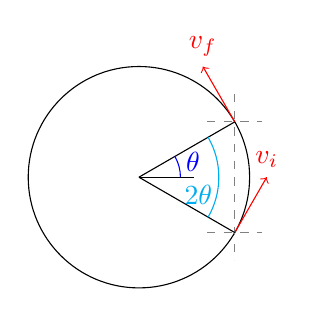
\begin{tikzpicture}
    \draw (0,0) circle(4em);

    % Velocity vectors
    \draw[->,color=red] (3.46410162em,2em) -- (2.3094em,4em) node[above]{\(v_f\)};
    \draw[->,color=red] (3.46410162em,-2em) -- (4.6188em,0) node[above]{\(v_i\)};

    % Vertical dashed line
    \draw[dashed, color=gray] (3.46410162em,3em) -- (3.46410162em,-3em);

    % Horizontal dashed lines
    \draw[dashed, color=gray] (2.46410162em,2em) -- (4.46410162em,2em);
    \draw[dashed, color=gray] (2.46410162em,-2em) -- (4.46410162em,-2em);

    % Angle reference lines
    \draw (0,0) -- (2em,0);
    \draw (0,0) -- (3.46410162em,2em);
    \draw (0,0) -- (3.46410162em,-2em);

    % Angle labels
    \draw[color=blue] (1.5em,0) arc(0:30:1.5em) node[midway, right, xshift=-0.1em, yshift=0.15em] {\(\theta\)};
    \draw[color=cyan] (2.5em,1.44338em) arc(30:-30:2.88676em) node[left, xshift=0.5em, yshift=0.8em] {\(2\theta\)};
  \end{tikzpicture}
\end{center}

\def\rv{{\color{red}v}}
\def\rvf{{\color{red}v_f}}
\def\rvfx{{\color{red}v_{fx}}}
\def\rvi{{\color{red}v_i}}
\def\rvix{{\color{red}v_{ix}}}
\def\rvx{{\color{red}v_x}}
\def\bt{{\color{blue}\theta}}
\def\bdt{{\color{blue}\Delta\theta}}
\def\b2t{{\color{cyan}2\theta}}

By definition,

\begin{equation}
  a = \lim_{\Delta t \to 0} \frac{\Delta v}{\Delta t}
\end{equation}

Noticing that since there is no change in the y-component of \(\rvi\) and \(\rvf\), the acceleration in the y-direction is zero. Therefore, we only need to consider the x-component of the velocity. Thus:

\begin{equation*}
  a = a_x = \lim_{\Delta t \to 0} \frac{\Delta \rvx}{\Delta t} = \lim_{\Delta t \to 0} \frac{\rvfx - \rvix}{\Delta t}
\end{equation*}

By trigonometry, we can see that:

\begin{align*}
  \rvix &= \rv \sin\bt \\
  \rvfx &= -\rv \sin\bt
\end{align*}

And from the definition of angular velocity, we know that:

\begin{align*}
  \omega &= \frac{\bdt}{\Delta t} \\
  \omega &= \frac{\b2t}{\Delta t} \\
  \Delta t &= \frac{\b2t}{\omega}
\end{align*}

Now, work out the limit:

\begin{align*}
  a &= \lim_{\Delta t \to 0} \frac{-\rv \sin\bt - \rv \sin\bt}{\Delta t} \\
  a &= \lim_{\Delta t \to 0} -\frac{2\rv \sin\bt}{\Delta t} \\
  a &= -\lim_{\bt \to 0} \frac{2\rv\omega \sin\bt}{\b2t} \\
  a &= -\lim_{\bt \to 0} \rv\omega \cdot \frac{\sin\bt}\bt \\
  a &= -\rv\omega \cdot \lim_{\bt \to 0} \frac{\sin\bt}\bt \\
  a &= -\rv\omega \cdot 1 \\
  a &= -\rv\omega \cdot 1
\end{align*}

Now finally, since \(v = r\omega\), we can substitute for \(\omega\):

\begin{align*}
  a &= -v \cdot \frac{v}{r} \\
  a &= -\frac{v^2}{r}
\end{align*}

Now for completeness, this is actually the acceleration in the x-direction. In this case, the x-direction is towards the center of the circle, so the negative sign indicates that the acceleration is centripetal. But the magnitude of the acceleration is of course positive.
